\chapter{(Multi-)domain adaptation in neural machine translation} \label{chap:mdmt-review}
The domain mismatch problem is one of the main challenges in machine translation \citep{koehn17six} in which the test distribution (the target domain) is different from the train distribution (the source domain). Domain adaptation approaches address the problem with one target domain, while multi-domain adaptation aims to improve the performance of an NMT model in many domains. While the problem has been actively studied for a long time, MT (multi-)domain adaptation literature lacks a unified foundation. Several previous works aimed to disambiguate the notion of a domain in MT domain adaptation, such as \cite{Wees15Whats,Wees17Whats,Saunders21Domain}. The thesis of \cite{Saunders21Domain} gave us a good review of domain adaptation. \citet{Chu18asurvey} regrouped domain adaptation approaches into two main categories, including the data-centric group and the model-centric group but also forgot to mention their use case. Because none of the reviewed methods in \citet{Chu18asurvey} solved all the situations of the domain mismatch problem, it is essential to summarize which method solves which case. Furthermore, these works only provided a facet of multi-domain adaptation. In this chapter, we want to propose a complete overview of this problem. First, we point out four main cases in (multi-)domain adaptation. Then we use a unique mathematical framework to describe these situations. Finally, we match domain adaptation methods to each case creating a Cartesian coupling of a technique and its application case.

We divide this chapter into five sections. In Section ~\ref{sec:domain}, we would like to discuss how we usually define a domain, how translations differ between domains, and the importance of domain adaptation in real applications. In Section ~\ref{sec:multi-facet} we would like to regroup two notions, domain adaptation and multi-domain adaptation, then divide the problem MT (multi-)domain adaptation into four main sub-problems. We dedicate the four following sections to these sub-problems. In each of these sections, we review groups of approaches (data-centric or model-centric), according to \citet{Chu18survey}, that match the requirement of the corresponding problem.
\section{What is a domain?}
\label{sec:domain}
In a classical machine learning context such as the binary classification problem, \citet{Shai10A} defined a domain by a pair of a distribution $\mathcal{D}_x$ on the input space $\Omega_x$ and a labeling function $g: \Omega_{x} \rightarrow \{ 0,1 \}$. In machine translation context, the labeling function will be $g: \Omega_{e} \rightarrow \Omega_{f}$ where $\Omega_{e}$ and $\Omega_{f}$ are the set of sentences of the language $e$ and the language $f$ respectively. Denote 2 different domains, $\big( \mathcal{D}_e^S, g^S \big)$ and $\big( \mathcal{D}_e^T, g^T \big)$. Domain adaptation is required when we train a machine learning model (statistical or neural) with the data generated by $\big(\mathcal{D}_e^S, g^S \big)$ but apply it to the data generated by $\big(\mathcal{D}_e^T, g^T \big)$. In principle, there is no guarantee that the model performs well in the second domain. However, we could aim to exploit some sharing knowledge between the two domains; for example, \citet{Blitzer06Domain,Miller19simplified} explored pivot features, which are features that frequently occur in the two domains and similarly contribute to the predictions in both domains. This paradigm was applied to multi-domain machine translation in the work of \citet{Britz17effective}. However, \citet{Pham21revisiting} reevaluated the method with a wider range of domains and observed a low performance.

In the machine translation literature, "a domain is defined by a corpus from a specific source" \citep{koehn17six}. \citet{Wees15Whats,Wees17Whats} identified the following elements of a text which influence the translation the most.
\begin{itemize}
	\item Topic: the subject of the text such as medical, news, IT, or religious. A topic owns its particular vocabulary. These items can not be transferred between distant topics such as medical and religion.
	\item Genre: the purpose of the text such as education, talk, report, or instruction. It identifies groups of texts that share a common form of transmission, purpose, and discourse properties. We characterize genre by textual style, the structure of the text, etc.
\end{itemize}

\citet{Carpuat13domain} provided an essential insight into domain adaptation. The authors carefully analyzed the sources of error when translating in a new domain. They identified unseen words and senses as the primary sources of error. According to \citet{Carpuat13domain}, there are four kinds of mistakes that an SMT system makes when translating in a new domain:
\begin{itemize}
	\item SEEN: unseen words in the new domain,
	\item SENSE: unseen domain-specific translations for known words,
	\item SCORE: wrong preference for non-new-domain translations,
	\item SEARCH: search algorithm chooses wrong words.
\end{itemize}
These errors are detected by analyzing the word alignment component of an SMT model. However, NMT models do not use word alignments explicitly in their mechanism. Moreover, the attention mechanisms in NMT architectures are usually hypothesized to play the same role as word alignment components implicitly. Consequently, SEEN, SENSE, SCORE, and SEARCH errors have not been used to analyze the performance of an NMT model in an unseen domain.

Despite many specifications, domains share the same grammar of the corresponding language and a relatively large vocabulary. Furthermore, domains from similar topics such as medical and scientific can share many common domain-specific words. Domains from a similar genre, such as administrative, can share the same formality. Therefore, the data of one domain can be helpful to improve the performance of a NMT model in other domains. The problem of (multi-)domain adaptation is to best exploit the similarity between domains and the specialization for each domain. These two goals are contrary to each other but both essential for a (multi-)domain MT system.

Solving the MT (multi-)domain adaptation problem is essential for deploying MT in a real context. Machine Translation has applications in many sectors, such as translating legal documents, news, scientific documents, books, movie subtitles, etc. Every domain has its specific vocabulary, registers (formal or informal), and genres (e.g., talk, instruction). Therefore, tailoring MT models to a target domain is essential to achieve good translation in that domain. In practice, MT models (SMT\nomenclature[smt]{SMT}{Statistical machine translation}, NMT) trained with domain-related data always perform much better in the domain of interest than ones trained with the same amount of less relevant data \citep{Rico13domain, Saunders21Domain}. The more domain-relevant data is available, the better the MT system performs in the target domain. However, not every domain has enough data to train an MT model. Moreover, state-of-the-art models such as Transformer models will need millions of parallel sentence pairs to learn its parameters. Therefore, we have to work around the situation where there is very little or no data. Domain Adaptation aims to improve the performance of an MT model in low-resourced domains. Besides, multi-domain adaptation seeks to achieve the best performance in more than one domain. However, the domains of interest in multi-domain adaptation are not limited to be low-resourced domains. The motivation of having one model adapted to many domains is to optimize the storage, the training time, and deployment time. Having one model per domain increases the storage, the time retrieving a model, and thus the translation latency. Online translation services, such as Google Translate, Systran Translate, or DL Translate, have to translate text from any possible domain while minimizing the latency of translation to be beneficial. In conclusion, the variety of text between application fields requires domain adaptation, while fast and robust translation requires multi-domain adaptation.

\section{Machine translation (multi-)domain adaptation - a multi-faceted problem}
\label{sec:multi-facet}
\subsection{From domain adaptation MT to multi-domain adaptation MT}
\label{ssec:formulizaion}
Domain adaptation and multi-domain adaptation do not have same motivation as one focuses on low-resourced domain whereas the other focuses on adapting to as many as possible domains, they can however cast under one general framework. Formally, train instances are distributed according to a mixture $\mathcal{D}_e^S$ such that $\mathcal{D}_e^S(x) = \sum_{d=1}^{n_d} \lambda^{s}(d) \mathcal{D}_e^d(x)$, with $\{\lambda^{s}(d), d=1 \dots n_d\}$ the mixture weights satisfying $\sum_d \lambda^{s}(d)=1$. The target domains are represented in the test distribution which is also a mixture of $\mathcal{D}_e^T(x) = \sum_{d=1}^{n_d} \lambda^{t}(d) \mathcal{D}_e^d(x)$, with $\{\lambda^{t}(d), d=1 \dots n_d\}$ the mixture weights satisfying $\sum_d \lambda^{t}(d)=1$. Domain adaptation solves the case where $\lambda^t$ is an one-hot vector while multi-domain adaptation happens to solve the case where $\lambda^t$ is not an one-hot vector. We illustrate this formulation in figure \ref{fig:mdmt-lambdas}.
\begin{figure}[h]
  \centering
  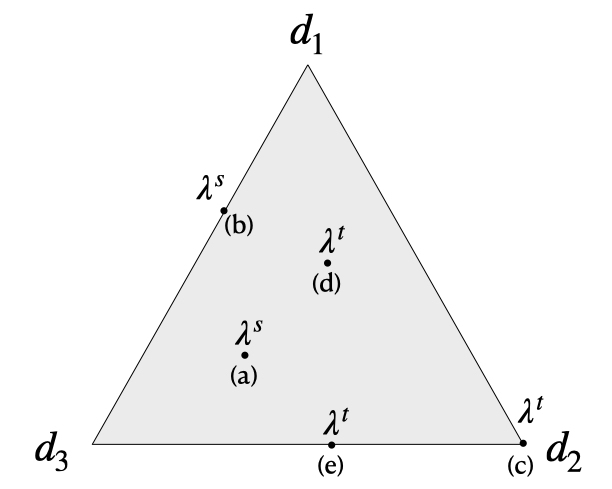
\includegraphics[width=0.5\textwidth]{graphics/mdmt-lambdas}
  \caption[Training and testing with distribution mismatch]{Training and testing with distribution mismatch. We consider just three domains, and represent vectors of mixture weights $\vlambda^{s}$ and $\vlambda^{t}$ in the 3-dimensional simplex. Training with weights in (a) and testing with weights in (c) is supervised multi-source domain adaptation to domain~2 ($d_2$), while (b)-(c) is the unsupervised version, with no train data from $d_2$; training with weights in (a) and testing with weights in (d) is multi-domain learning, also illustrated with configurations (a)-(e) (train domain $d_1$ is not seen in test), and (b)-(d)  (test domain $d_2$ is unseen in training).}
  \label{fig:mdmt-lambdas}
\end{figure}

This framework describes the real context closely because, in a typical setting in machine translation, we collect the most extensive collection of parallel data for the chosen language pair to achieve optimal performance for the task of interest. In such situations, the train data's distribution is opportunistic. The test data distribution is also a pre-determined mixture of the target domains. A key objective in training (multi-)domain NMT models is to mitigate the detrimental effects of a possible mismatch between these distributions. 

Train data may be a mixture of many domains such as the JRC-Acquis Communautaire corpus (\domain{law}-domain) \citep{Steinberger06acquis} or documentation for KDE, Ubuntu, GNOME and PHP from the Opus collection \citep{Tiedemann09news} (\domain{it}-domain). We can also leverage a collection of data with no specific topic and genre, such as Paracrawl \citep{Banon20Paracrawl}, for example in \citet{nathan19facebook}. 

In (multi-)domain adaptation, the test data is a mixture of target domains. The weight of each target domain in the mixture is proportional to the priority of the domain. Empirically, test data consists of the test sets of the target domains. The performance of an MT system is the average of its performance on these tests weighted by domain weight in the mixture. Most of papers use uniform weights. However, we can assess the quality of a multi-domain MT system with different priorities over the target domains using weighted mean.

\subsection{Four main sub-problems}
\label{ssec:4cases-chap3}
From our study of the literature of (multi-)domain adaptation, we realize that all the cases of (multi-)domain adaptation can be classified into four groups by answering two following questions:
\begin{itemize}
	\item Is/Are the train domain(s) determined?
	\item Is/Are the test domain(s) determined?
\end{itemize}
More precisely, the first question asks whether the train data is composed of a number of known domains. For example, the domain of a mixture of multiple corpora of specific topics, such as JRC-Acquis Communautaire corpus (\domain{law}-domain) and KDE (\domain{it}-domain), is well defined. However, the domains in Paracrawl \citep{Banon20Paracrawl} are unknown because the corpus was built by crawling the content of web-sites without specifying topic or purpose. The second question asks whether the domain of the test data is determined. If there exists a collection of text (monolingual or parallel) that defines the test domain, then it is domain-determined and vice versa.

The first case of (multi-)domain adaptation, which will be presented in Section ~\ref{sec:case1}, is supervised multi-domain adaptation in which domain labels are both available in training and testing. The format of train data is the triple $(d,x,y)$, in which $d$ is the index of the domain, $(x,y)$ is a pair of parallel sentences. The format of test data is $(d,x)$. This case might be the most straightforward situation. Many studies have been conducted in this setting \citep{Pham21revisiting}.

The second case that we discuss in Section ~\ref{sec:case2} considers the use of the parallel data crudely collected from web sites such as Paracrawl \citep{Banon20Paracrawl} or Commoncrawl \footnote{\url{https://commoncrawl.org/}}. The content of these corpora is a mixture of many topics, but unfortunately, there is not any available domain label for sentences. Fortunately, in this second case, the target domains are known, i.e., there exist data for these domains, which can be used to adapt the model. The format of train data will be $(?,x,y)$. The format of test data will be $(d,x)$. This case focuses on the exploitation of opportunistic text. 

The third case in Section ~\ref{sec:case3} assumes a well domain-labeled train data, whereas the test data can come from any possible domain. This case focuses on the robustness of the MT system against any potential shift distribution in testing. The format of train data is $(d,x,y)$. The format of test data is $(?,x)$. The third setting is very close to most translations on the web, where the provenance of the input text is unknown. 

Finally, the last setting in Section ~\ref{sec:case4} focuses on both exploiting opportunistic data in training and being robust against unknown test distribution. The format of train data is $(?,x,y)$. The format of test data is $(?,x)$. We dedicate the four following sections to discuss each setting more thoroughly.

Recently the work of \citet{Chu18survey} attempted to describe the landscape of MT domain adaptation by categorizing previous methods in 2 main classes: data-centric and model-centric. The data-centric category includes methods that manipulate the train distribution to resemble the distribution of the target domain better. The model-centric methods focus on changing the architecture, modifying the train objective, and improving the inference. \citet{ramponi20neural} also adopted this taxonomy in their survey on unsupervised domain adaptation in natural language processing.

According to \citet{Chu18asurvey}, the data-centric methods focus on two paradigms, including 1) collecting parallel data related to the domain target, 2) creating synthetic data resembling the domain target. The first paradigm searches for similar examples to the ones of the domain target to enlarge the target domain's train data. The second paradigm aims to create pseudo samples resembling the data of the domain target. Besides the two paradigms, we propose another paradigm, which is data sampling. The data sampling paradigm consists of changing the data sampling scheme during the training course to mitigate the heterogeneity of the data size between domains and the variety of the "difficulty" of the domains. The data-centric group consists of 2 paradigms, including 1) data sellection, 2) data synthesis.

This taxonomy is primarily adopted in MT domain adaptation's research. However, we find a naivety in this classification as it misses delivering an answer for the most ultimate question: "which method solves which problem?". The four following sections will explain how the model-centric and the data-centric categories solve 4 (multi-)domain adaptation cases. We also introduce several adaptation problems that need more research effort and other applications of existing methods. The work of \citet{Pham21revisiting} recently gave a brief review of several well-known adaptation methods via a reevaluation with different domain adaptation cases. However, the experiments are still limited in the first case \ref{sec:case1} and the third case \ref{sec:case3} as they excluded non-domain-determined train data such as crawled corpora in their experiments.

\section{Supervised (multi-)domain adaptation}
\label{sec:case1}
In the supervised (multi-)domain adaptation problem, the domain label is available in both the train data and the test data. Furthermore, the domain(s) in the test data is(are) included in the train data. In this problem, we would like to train a single model that performs the best in our target domains, given train data from those domains and probably from other domains. This setting is the most popular adaption problem in the literature. This first case represents the easiest requirement for an MT model. A model needs to achieve the best performance on the domains of its train data. The difficulty of this situation is to both exploit the proximity between domains while mitigating the interference due to inter-domain heterogeneity. Effectively, similar topics, such as \domain{legal} and \domain{administrative}, might improve the vocabulary coverage of each other as both domains share the same domain-specific words. However, distant topics, such as \domain{religion} and \domain{IT} might confuse the NMT system when sharing the same parameters. In the following sections, we will discover how model-centric methods and data-centric methods solve this case.
\subsection{Model-centric approaches}
In the case of supervised multi-domain adaptation, model-centric methods focus on adding domain-specific parameters to reduce the interference between domains while keeping the total number of parameters small. The simplest approaches use domain tags. For example, \citet{Kobus17domain} proposed appending a special token to each source sequence indicating its domain such as $<Domain=IT>$ and train the NMT model with this input. However, this method requires the domain tag of a sentence before translating it. Therefore, we have to predict the domain tag of the source sentence if it is from an unknown origin. \citet{Britz17effective} originally proposed appending domain tag to the target sequence so that the decoder will predict the domain in which it will generate the translation. Instead of using domain tags, \citep{Kobus17domain} proposed using domain embeddings to incorporate the domain information into the context of the translation. \citet{Kobus17domain} concatenated a domain embedding of small size (e.g., 4) to the embedding of each token in the input sequence. Each domain has its own embedding. Instead of using the domain embedding to represent the domain in the representation, \citet{Pham19generic} used a sparse word embedding called "lexicalized domain representation", in which a number of dimension are reserved for one domain and will be nullified if the model translates in other domains. We will discuss more this method in Chapter ~\ref{chap:ldr}. Besides domain embeddings, it is possible to use domain-specified layers that can be plugged between 2 consecutive layers of the NMT model without changing the architecture. There are 2 types of plug-in layers: 1) residual adapters \citep{Bapna19simple, Pham20Study} and 2) hidden unit contribution layers \citep{Vilar18learning}. Residual adapters were first introduced by \citet{Rebuffi17learning} in computer vision. \citet{Bapna19simple} proposed this fine-tuning paradigm for domain adaptation and for multilingual NMT. They introduced a variant of residual adapters introduced in \citet{Rebuffi17learning} composed of 2 linear projections and $ReLU$ activation function. The adapters are plugged into the NMT model as follows
\begin{equation}
\begin{array}{rcl}
h_{enc/dec}^l = h_{enc/dec}^{l} + ADAP_{enc/dec}^l(h_{enc/dec}^{l})
\end{array}
\end{equation}
where $ADAP_{enc/dec}^l$ is the adapter corresponding to the $l^{th}$ layer of the encoder/the decoder. \citet{Pham20Study} studied the use of the residual adapters for multi-domain adaptation and propose several techniques, including the regularization, a gating mechanism, to improve the robustness of the model. They will be presented in Chapter ~\ref{chap:res}. The hidden unit contribution layers (LHUC \nomenclature[lhuc]{LHUC}{Learning hidden unit contribution}) were proposed by \citet{Vilar18learning} to adapt an NMT model to a domain. The author applied an LHUC layer to the model as follows
\begin{equation}
h_{enc/dec}^l = h_{enc/dec}^{l} \odot a(\rho^{l}_{enc/dec})
\end{equation}
where $\rho^{l}_{enc/dec}$ is the adapter corresponding to the $l^{th}$ layer of the encoder/the decoder and $\rho^{l}_{enc/dec} \in \mathbb{R}^d$. $a(.)$ is a scaled
element-wise sigmoid function.
$$a(x) = \frac{2}{1+e^{-x}}$$
Residual adapters and LHUC layers adapt a pretrained model without changing its parameters. 

While the previous methods aim to discriminate domains to reduce the interference, \citet{Britz17effective} were motivated to learn hidden representations that are invariant between domains. More precisely, the authors use a binary classifier that takes the output of the encoder as input to predict the domain of the source sequence. They inverse the sign of the gradient with respect to the loss of the classifier to confuse it, i.e., making the hidden representation of the encoder invariant between 2 domains. This technique is related to A-distance, which is a measure of similarity between two probability distributions. \citet{Ben07analysis} showed that the A-distance between the source and target distributions is a crucial part of an upper generalization bound for domain adaptation. The authors hypothesized that it should be difficult to discriminate between the source and target domains to transfer between them well. \citet{Zeng18multidomain}'s work was also inspired by this idea. However, instead of forcing the encoder's output to be invariant between domains, the authors aimed to extract domain-agnostic features and domain-specific features from the output of the encoder and feeding these features to the decoder. To this end, they used two different non-linear transformations, which map the output of the encoder to two feature vectors of the same size. Then, they applied a domain classifier on each feature vector. The domain-agnostic feature vector is trained to confuse the classifier, whereas the domain-specific feature vector is trained to facilitate its classifier.

\citet{Michel18extreme} adapted a pretrained model to a multi-user personalized model by fine-tuning the bias of the output layer to each particular user of the MT system. The number of additional parameters is $|S| \times |\Sigma_y|$, in which $S$ is the set of the users. The authors reduced the size of the bias matrix $B \in \mathbb{R}^{|S| \times |\Sigma_y|}$, where each row is bias vector for one user, by factoring it into lower dimension representation, i.e.
\begin{equation}
\begin{array}{rcl}
B &=& S \times \tilde{B}, \\
&where& \\
S & \in & \mathbb{R}^{|S| \times r}, \\
\tilde{B} & \in & \mathbb{R}^{r \times |\Sigma_y|}.
\end{array}
\end{equation}

\citet{Jiang20Multi}'s work was inspired by the mixture of expert paradigm. Their model is based on the Transformer architecture \citep{Vaswani17attention} as they integrate a domain-mixing mechanism to the multi-head attention layer. As we explained in Section ~\ref{ssec:transformer-enc}, each head of a multi-head attention layer is computed as follows
\begin{equation}
head_i = Attention \big(QW_i^Q, VW_i^V, KW_i^K \big).
\end{equation}
Suppose that there are $K$ domains: at the $i^{th}$ head, for the query, the key and the value components, there are $K$ transformation matrices $W_{i,j}^Q | j \in [1,K]$, $W_{i,j}^K | j \in [1,K]$, $W_{i,j}^V | j \in [1,K]$ respectively. The domain-mixing mechanism is applied to the query, the key and the value components as follows
\begin{equation}
\begin{array}{rcl}
Q_i^t &=& \sum_{j=1}^K Q^tW_{i,j}^Q*\mathit{D}_j(x_t),\\
K_i^t &=& \sum_{j=1}^K K^tW_{i,j}^K*\mathit{D}_j(x_t),\\
V_i^t &=& \sum_{j=1}^K V^tW_{i,j}^V*\mathit{D}_j(x_t),\\
head_i &=& Attention \big( Q_i, K_i, V_i\big),
\end{array}
\end{equation}
where the subscript $t$ indicates the position of the vector in the sequence of hidden representations, $\mathit{D}(x_t) \in \mathbb{R}^{K}$ is the domain proportion of the corresponding token $x_t$. The proportion of domains of a token is computed by a domain classifier, that takes the input embedding of that token as input. By doing this, the model adapts the hidden representation of a token to the domain to which the token likely belongs. Consequently, the model is able to discriminate domains for domain-specific tokens while transferring knowledge between domains for domain-agnostic tokens. However, the size of the model is proportional to the number of domains, which is not practical in the real applications. The idea can be applied to residual adapters or LHUC layers.

Recently, \citet{Gong21pay,Gong21adaptive} proposed learning domain-specific head selections in the multi-head attention mechanism to mitigate the interference between domains/languages. The authors used a variational NMT model with discrete latent variables $z^{(h)}_t$ from a Bernoulli distribution indicating whether a task $t$ selects the attention head $h$. The training jointly learns the NMT model and the inference networks $q_{\theta^{(h)}_t}(z)$ of the pairs of (task $t$, head $h$) by optimizing the evidence lower bound (ELBO) \citep{kingma13variational} with Gumbel-softmax reparametrization trick \citep{jang17categorical}.

Besides the model-centric methods related to the architecture, multi-task training is another solution to the supervised (multi-)domain adaptation problem. 

We illustrate several well-known model-centric methods for the supervised domain adaptation problem in figure~\ref{fig:model-centric-case1-case2}.
\begin{figure}[htbp]
\begin{subfigure}{1.0\textwidth}
  \centering
  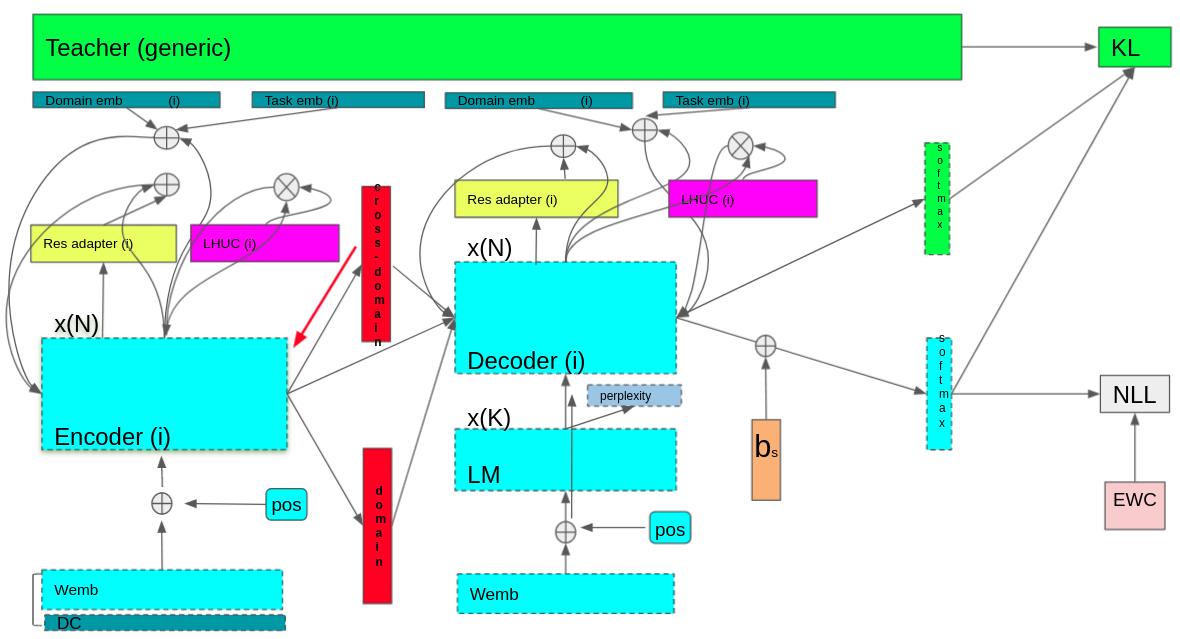
\includegraphics[width=1.0\textwidth]{graphics/supervised_mdmt}
\end{subfigure}
\newline
\begin{subfigure}{1.0\textwidth}
  \centering
  \fbox{\begin{tabular}{ll}
 
\textcolor{darkcornflowerblue}{$\blacksquare$} & \citet{Kobus17domain} \\
\textcolor{darkblue}{$\blacksquare$} & \citet{Dou19unsupervised} \\
\textcolor{yellow}{$\blacksquare$} & \citet{Bapna19simple} \\
\textcolor{red}{$\blacksquare$} & \citet{Zeng18multidomain} \\
\textcolor{magenta}{$\blacksquare$} & \citet{Vilar18learning} \\
\textcolor{green}{$\blacksquare$} & \citet{Dakwle17fine} \\
\textcolor{lightorange}{$\blacksquare$} & \citet{Michel18extreme} \\
\textcolor{lightred}{$\blacksquare$} & \citet{Brian19overcoming} \\
\end{tabular}}
\end{subfigure}
\caption[Model-centric's brief overview]{Each color except the blue corresponds to one model-centric method. The blue represents the NMT model.}
\label{fig:model-centric-case1-case2}
\end{figure}

\subsection{Data-centric methods}
\subsubsection{Data sampling}
In supervised multi-domain adaptation, data sampling approaches aim to balance the contribution of each domain to the final model. In multi-domain train data collected opportunistically, the data size of each domain varies from few thousands examples to millions examples. In a trivial mixture of data, small domains are usually excessively under-sampled causing a sub-optimal performance in average. However, if we equally sample data from every domain, the NMT model is easily over-fitted in the small domains. Therefore, finding an optimal sampling scheme across domains is essential. \citet{Wang20balancing} proposed parameterizing the probability of sampling data from a domain and learned this probability via REINFORCE algorithm \citet{Williams92simple} using rewards computed from the cosine-similarity between the gradient over in-domain train data and the gradient over dev-sets' data. We compare this technique to our approach in Chapter ~\ref{chap:mdac}\fyDone{add reference of chapter MDAC here}.

Other data-centric methods, that do not take into account the domains of the train data will be discussed in Section ~\ref{ssec:case-2-data}.
\section{Undetermined train domain, determined test domain}
\label{sec:case2}
In this situation, the train data is composed by an unknown number of domains. The second case focuses on adapting the NMT model with an unknown source domain while the target domain is well defined. There are two situations: 1) there exists parallel data in the target domain 2) there exists only monolingual data in the target domain. The two following sections will discuss how each group of method solves these cases.
\subsection{Model-centric methods}
First, we discuss the case with one target domain in which there exist parallel data. In this case, we can apply the same techniques proposed for supervised (multi-)domain adaptation by considering the source domain as a generic domain. Besides, fine-tuning is a very efficient approach for this problem\citep{Luong15stanford,Servan16Domain,Freitag16fast,Miceli17regularization}. We first train an NMT model with the mixture of source domains, then continue training this model with the parallel data of the target domain. According to a recent review of multi-domain adaptation conducted by \citet{Pham21revisiting}, fine-tuning is the strongest baseline in supervised domain adaptation. However, fine-tuned NMT models usually suffer from catastrophic forgetting \citep{Michael89catastrophic} as their performances drop dramatically in the source domains. To mitigate the catastrophic forgetting, several regularization techniques were introduced, including mixed fine-tuning \citep{Chu17empirical}, uniform weight-decay \citep{Miceli17regularization}, elastic weight consolidation (EWC \nomenclature[ewc]{EWC}{Elastic weight consolidation}) \citep{Kirk16overcoming,Brian19overcoming,Saunders19domain} and knowledge distillation \citep{Dakwle17fine}. 

Mixed fine-tuning \citep{Chu17empirical} adapts an NMT model with the mixture of the source domain and the target domain (by oversampling the target domain). The method adapts the NMT model to the domain of interest thanks to the oversampling while maintaining its robustness to generic text as it continues to be trained with the source domain.

Weight decay \citep{Miceli17regularization} continues training the NMT model on the target domain's data with a regularized loss 
\begin{equation}
L_{CE}(\theta, \mathcal{D}^t_e, g^t) + \alpha * \parallel \theta - \theta^{A} \parallel_{L_2},
\end{equation}
where $\theta^{A}$ is the value of the pretrained model, $\mathcal{D}^t_e, g^t$ characterize the target domain $t$. Fine-tuning with the new loss fits the model to the target domain while preserving the the old pretrained parameter values, therefore preventing the overfitting of the NMT model in the target domain and maintaining the generality over source domains. \citet{Kirk16overcoming, Brian19overcoming, Saunders19domain} were also motivated to penalize the changes of the parameters compared to the initial model. However, the authors argued that not every parameter has the same contribution to maintain the generality to the old domains and that we can tune the parameters unimportant for the old domains to the target domain. The contribution of each parameter of the pretrained model is approximated by the diagonal of the Fisher matrix computed over the data of the source domains. Fine-tuning with EWC uses the following loss
\begin{equation}
L_{CE}(\theta, \mathcal{D}^t_e, g^t) + \sum_{i} \frac{\lambda}{2} F_i * (\theta_i - \theta_i^{A})^2,
\end{equation}
where the $F_i$ is the $i^th$ element of the diagonal of the Fischer matrix approximated as follows
\begin{equation}
\bar{F} = E_{x \sim \mathcal{D}_e^s(x), y \sim g^s(x)} \big[ \nabla logP(y|x,\theta)_{| \theta^{A}} \nabla logP(y|x,\theta)_{| \theta^{A}}^{T} \big],
\end{equation}
in which $\mathcal{D}^s_e, g^s$ characterize previous train domains.
\citet{Dakwle17fine}'s method was motivated by the knowledge distillation paradigm \citep{Hinton15Distilling}. The authors proposed regularizing the standard cross-entropy loss with the Kullback-Leibner distance \citep{Kullback51On} between two predicting distributions produced by the old model and the new model as follows
\begin{equation}
L_{CE}(\theta, \mathcal{D}^t_e, g^t) + \alpha * E_{x \sim \mathcal{D}_e^s(x), y \sim g^s(x)} \big[ KL(P(.|x,\theta) | P(.|x,\theta_{A})) \big],
\end{equation}
in which $\mathcal{D}^s_e, g^s$ characterize previous train domains.
Instead of continuing training with target domain only, \citet{Chen17cost} differentiated directly domain-relevant instances and irrelevant instances via instance weighting. The authors compute the weight of each instance by a domain classifier, that is trained with source sequences. The training will maximize the following objective 
\begin{equation}
\begin{array}{rcl}
\hat{\theta} = \displaystyle{\mathop{\arg max}_{\theta}} E_{x \sim \mathcal{D}_e^s(x), y \sim g^s(x)} (1+p_d(x))log(P(y|x,\theta)) + E_{x \sim \mathcal{D}_e^t(x), y \sim g^t(x)} (1+p_d(x))log(P(y|x,\theta))
\end{array}
\end{equation}
where $\mathcal{D}_e^t, g^t$, $\mathcal{D}_e^s, g^s$ are the target domain and other domains, $p_d(x)$ is the probability that $x$ comes from the target domain. \citet{Wang17instance} proposed using different domain-relevance metrics for instance weighting. 

Besides methods using auxiliary losses, ensemble methods are also promising. For example, \citet{Freitag16fast} proposed ensembling the pretrained model and the fine-tuned model to combine the advantage of both models: the specialization in the target domain and the generalization over general text.

Still in the case of uni-domain adaptation, but without parallel data, the model-centric approaches mostly use monolingual data in the target language of the target domain. The proposed methods mostly adapted the decoder to the target domain. For example, \citet{Gulcehre16monolingual} proposed training a language model adapted to the target domain and fusing the language model to the decoder. The fusion could be deep or shallow. The deep fusion combined the hidden representation of the decoder and the one of the language model before computing the prediction probability. The shallow fusion combined the prediction probability computed by the decoder and the one computed by the language model. \citet{Domhan17using} was also motivated by this idea. However, the authors proposed jointly training the language model and the NMT model via multi-task training. Furthermore, the decoder and the language model shared the word embedding of the target side.

All previous methods were motivated to adapt an NMT model to a specific domain. We realize that they can hardly be applied to multi-domain adaptation because all the parameters of the MT model are adapted to one domain. However, in the case where there are parallel data of the target domains, we could use model-centric methods proposed in the supervised adaptation by considering the train domain a generic domain. Recently, \citet{Dou19unsupervised} proposed using domain embeddings and task embeddings to adapt an NMT model to the target domain using reconstruction loss on the monolingual data. More precisely, for each layer $l^{th}$ of an ANMT model, there are 2 task embeddings $\theta_{task}^{\gamma,l}$, $\gamma \in \{ MT, LM \}$, which correspond to translation task and language modeling task respectively. Furthermore, for each layer $l^{th}$, and for each domain $d$, there is a domain task $\theta^{d,l}_{dom}$. The layer $l^{th}$ of encoder/decoder will be as follows
\begin{equation}
h^{l} = LAYER^l(h^{l_1}) + \theta^{d,l}_{domain} + \theta_{task}^{\gamma,l}
\end{equation}
Now, the parallel data will be used to compute the translation loss, while the monolingual data is used to compute the language modeling loss. The authors proposed adding noises to the source sequence while computing the LM loss. Using domain-specific embeddings enables the model to be adapted to multiple domains at once. Despite being applied to multi-lingual machine translation, the monolingual adapter proposed by \citet{Philip20monolingual} shares the same spirit and can be applied to this situation.
\subsection{Data-centric approaches}
\label{ssec:case-2-data}
According to our study, the previous data-centric approaches proposed to this situation belong to all three paradigms, including data selection, data synthesis, and data sampling. The two following sections will discuss the methods of each paradigm.
\subsubsection{Data selection}
Data selection approaches collect parallel data, which resemble the target domain. The selection is usually based on a score of proximity between a parallel example and the domain. The score of proximity can be computed via sentence embeddings or variants of \citet{Moore10intelligent} score. For example, given two corpora of a target domain $D_{I-src}$, $D_{I-tgt}$ and two corpora of the source domain $D_{O-src}$, $D_{0-tgt}$, \citet{Axelrod11domain} computed a bilingual version of Moore $\&$ Lewis score of a sentence pair as follows
\begin{equation}
\begin{array}{rcl}
S_{bi} (x,y) &=& H_{I-src}(x) - H_{O-src}(x) + H_{I-tgt}(y) - H_{O-tgt}(y), \\
\end{array}
\label{eq:ced}
\end{equation}
where the cross-entropy $H_{*}(z)_{| * \in [I-src, I-tgt, O-src, O-tgt], z \in [x,y]}$ of the sentence $z$ is computed by a language model trained only with the corpus $D_{*}$. \citet{Duh13adaptation} proposed the same formulation as proposed \citet{Axelrod11domain} but used a neural language model instead of a statistic language model. In a survey of data selection methods for neural machine translation, \citet{Silva18extracting} evaluated 3 popular methods in the domain adaptation task, including the cross-entropy difference, the Term Frequency-Inverse Document Frequency embeddings (TF-IDF \nomenclature[tf-idf]{TF-IDF}{Term Frequency-Inverse Document Frequency}) \citep{Salton73On} and the Feature Decay algorithm (FDA \nomenclature[fda]{FDA}{Feature Decay Algorithm}) \citep{Poncelas18Feature}. More precisely, the cross-entropy difference was computed as described above and normalized by sentence length. To compute a TF-IDF representation vector, \citet{Silva18extracting} consider each sentence of the target domain as a query and every sentence in the source domain as a key. The tf-idf vectors of the queries and the keys are computed as in \citet{Salton73On}. The score of proximity between a query and a key is the cosine-similarity of theirs tf-idf vectors. Based on the score of proximity, for each sentence of the target domain, we retrieve K nearest-neighbors in the source domain. The collection of the retrieved sentences is the result of the method. Finally, FDA aims to extract from train data a set of sentences that are most relevant to the test set of the target domain. We call an extracted n-gram a feature. The method extracts n-grams from the source side of the test set. In the beginning, the features are assigned the same value. Each sentence of the train data is scored as the normalized (by dividing by the number of words) sum of the values of its features. Then, the method selects the sentence with the highest score and adds it to the set of selected data (which initially is empty). After selecting a sentence, the values of the features contained in it are decreased. The decay function is defined as follows
\begin{equation}
decay(f) = init(f) * 0.5 ^{C_{L}(f)},
\end{equation}
where $f$ is an n-gram, $init(f)$ is the initial value assigned to each feature and $C_{L}(f)$ is the count of the feature $f$ in the selected data.

\citet{Wang17sentence} proposed using a sentence embedding to represent a sentence instead of a $tf-idf$ vector. For each language side (source/target) the authors computed the centroid of the target domain and one of the source domain. Assume $C_{E_{in}}$, $C_{E_{out}}$ are the centroid of the target domain and the source domain in the source language,  $C_{F_{in}}$, $C_{F_{out}}$ are the centroid of the target domain and the source domain in the source language, $v_{\mathit{e}}$ is the sentence embedding of a source sentence $\mathit{e}$, $v_{\mathit{f}}$ is the sentence embedding of a source sentence $\mathit{f}$, then the proximity of the example $(\mathit{e},\mathit{f})$ to the target domains is defined as follows
\begin{equation}
d(v_{\mathit{e}}, C_{E_{in}}) - d(v_{\mathit{e}}, C_{E_{out}}) + d(v_{\mathit{f}}, C_{F_{in}}) - d(v_{\mathit{f}}, C_{F_{out}}),
\end{equation} 
where $d(.,.)$ is the Euclidean distance in $\mathbb{R}^d$. \citet{Aharoni20unsupervised} proposed using sentence embeddings computed by a pretrained Bidirectional Encoding Representation Transformer (BERT \nomenclature[bert]{BERT}{Bidirectional Encoding Representation Transformer}) and the cosine-similarity to retrieve domain-related examples.

\subsubsection{Data synthesis}
The most efficient approach in this paradigm is backtranslation \citep{Sennrich16improving}, which consists of translating the monolingual data of the target language to the source language. \citet{Burlot18using} showed significant improvement of an NMT model in the target domain when trained with a mixture of parallel data and in-domain backtranslated data. Without backtranslating the target-side data, \citet{Currey17copied} created artificial sentence pairs from the monolingual data in the target language so that each source sentence is identical to the target sentence. Training an NMT model with the mixture of parallel data and artificial sentences improves the accuracy of the translation on named entities and other words that should remain identical between the source and target languages. Recently \citet{currey20distilling} proposed distilling knowledge from multiple domain experts to a multi-domain NMT model. The authors translated each source side in-domain corpus with the corresponding adapted model, then mixed the artificial corpora to the train corpora and continued training the multi-domain NMT model with the new corpora.

\subsubsection{Data sampling}

Data sampling methods dynamically change the composition of the train data over time. In practice, the evolution of the train data is beneficial for training an NMT model specialized to a domain. For example, in the fine-tuning approaches, the training begins with every available data and finishes with the data of the target domain. Data sampling methods consist of building an automatic curriculum without human supervision. For example, \citet{Wees17dynamic} proposed gradual fine-tuning, which first computes a sampling distribution based on the cross-entropy difference (CED) \eqref{eq:ced} of each example, then gradually decreases the number of sampled examples after each epoch. Formally, the CED score of each example is normalized as follows
\begin{equation}
\tilde{CED}(x) = 1 - \frac{CED(x)-min(CED_{G})}{max(CED_{G}) - min(CED_{G})},
\end{equation}
where $G$ is the train corpus. Therefore higher-ranked examples have a higher $\tilde{CED}$ score rather than having lower $CED$ as in \citet{Axelrod11domain}. The sampling distribution is computed as follows
\begin{equation}
\omega(x) = \frac{\tilde{CED}(x)}{\sum_{x'\in G} \tilde{CED}(x')}.
\end{equation}
For each epoch $i^{th}$, a number $n_i$ of examples are selected according to the previous distribution. $n_i$ is defined as follows
\begin{equation}
n_i = \alpha \cdot |G| \cdot \beta^{\lfloor \frac{i-1}{n}, \rfloor}
\end{equation}
where $\alpha \in [0,1]$ is the relative start size, $\beta \in [0,1]$ is the retention rate. Via the same mechanism, \citet{Wang19dynamically} proposed a more sophisticated dynamical sampling scheme combining two scores of an example, $domain-CED$ and $noise-CED$. The authors proposed two variants: mixed co-curriculum, which scores an example by the sum of its $CED$ scores, and cascaded co-curriculum, which first selects examples by their $domain-CED$ scores then retains top examples according to their $noise-CED$ scores from the previous selection. Furthermore, \citet{Wang19dynamically} proposed to recompute the language model of the noisy data for each epoch. Instead of increasing the domain-relevance of the train data, \citet{Zhang19curriculum} did the opposite. More precisely, they reordered the train data according to their relevance to the target domain then equally split the whole corpus into many shards containing samples of a similar score. They trained an NMT model with one shard per epoch in a decreasing order of domain-relevance.

Besides well-known metrics for domain-relevance, \citet{Zhang19curriculum} proposed a parameterized scorer, that evaluates the usefulness of each sample to the performance on the target domain, and optimized its parameters via Bayesian optimization. More precisely, the scorer was formulated as follows
\begin{equation}
\mathit{f}(x,y) = V \cdot \mathbf{F}(x,y),
\end{equation}
where the feature vector $\mathbf{F}(x,y)$ was extracted from the example, and the weight vector $V$ was learned by Bayesian optimization. Each element in $\mathbf{F}(x,y)$ represents the relevance of the example to a target domain. Once the scorer was optimized, the training was conducted as in \citet{Wees17dynamic,Wang19dynamically}.

\section{Determined train domain, undetermined test domain}
\label{sec:case3}
The third case is interesting because it resembles the real context of machine translation's applications. Effectively, the users' text can be from any possible topic or for any possible purpose (genre). In this situation, the NMT model needs to be both robust to the unseen domains and adapted to known domains. 
\subsection{Model-centric methods}
Mixture models are a promising solution for this situation as they combine domain-adapted systems to perform the translation. Effectively, the performance of mixture models is guaranteed in the source domains while using a convex combination of the adapted systems is robust against unseen domains. Mixture models have been successfully applied for SMT models \citep{Sennrich12mixture,Sennrich12perplexity,Carpuat14linear}. \citet{Freitag16fast, Sajjad17neural, Saunders19domain} applied mixture models to NMT models. The contribution of each adapted model to the combination was uniform in \citet{Freitag16fast} while \citet{Sajjad17neural} pre-finetuned the weights by Bayesian optimization on a development set. However, a heuristic static weights are sub-optimal when the test domain is highly variable. \citet{Saunders19domain} proposed computing the weights of the mixture for each source sentence $x$ at the $i^{th}$ decoding step as follows
\begin{equation}
\begin{array}{rcl}
W_{k,i} &=& \displaystyle{\mathop{\sum}_{t} P(t=k|h_i,x)\lambda_{k,t}}, \\
&where& \\
P(t=k|h_i,x) = P(t=k|x) &=& \frac{\displaystyle{P^k_{LM}(x)}}{\displaystyle{\mathop{\sum}_{k'} P^{k'}_{LM}(x)}},\\
\end{array}
\end{equation}
where $P^{k'}_{LM}(x)$ is the probability of the source sentence $x$ according to a language model learned from domain $k'$, $\lambda_{k,t}$ can be uniform, identity or pre-finetuned with a development set. \citet{Saunders19domain} also proposed varying the mixture's weights during the inference by conditioning the domain posterior probability on both $x$ and $h_i$ as follows
\begin{equation}
P(t=k|h_i,x) = \frac{P(h_i|t,x) P(t|x)}{\displaystyle{\mathop{\sum}_{k'} P(h_i|k',x) P(k'|x)}}.
\end{equation} 
Besides one might be more interested in domain robustness than in domain specialization. The mixture model does not include the domain robustness in the training objective. \citet{Muller20domain} discussed several regularization methods to mitigate the problem, including the subword regularization \citep{Taku18subword}, the defensive distillation \citep{Papernot16distillation}, the reconstruction \citep{Tu17neural} and the neural noisy channel reranking \citep{Li16mutual}. The distributional robustness optimization \citep{BenTal13robust,Oren19distributionally} is also a promising paradigm as the related methods optimize models so that they perform well over a wide range of potential test distributions. However, the application of this paradigm to neural machine translation has not yet been explored.
\subsection{Data-centric methods} \label{ssec:data-centric}
The data-centric paradigm can not be applied to this situation since the domain of the test sentences is unknown. Indeed, the data-centric approaches aim to build train data that approximates a target domain and require the monolingual data of that domain to create the pseudo in-domain data. That can only be done when we know the target domain.
\section{Undetermined train domain, undetermined test domain}
\label{sec:case4}
\subsection{Model-centric methods}
\citet{Farajian17multidomain,Li18onesentence} proposed fine-tuning on-the-fly a pretrained model with a mini-batch similar to the source sentence before translating it. The authors chose the learning rate and the number of fine-tuning iterations according to the similarity score between the retrieved mini-batch and the source sentence so that the higher similarity the higher the learning rate, the more iterations. \citet{bulte19neural,bapna19non,Pham20Priming,xu20boosting} proposed learning an NMT model to reuse parallel examples whose source sentence is similar to the source sentence. Some of these techniques are discussed in Chapter ~\ref{chap:priming}.
\subsection{Data-centric methods}
The data-centric paradigm can not be applied to this situation for the same reason as in previous Section ~\ref{ssec:data-centric}

\section{Multi-domain and multi-lingual machine translation}
We can put multi-domain and multilingual machine translation under the same umbrella of multi-task learning where a task is one language pair or one domain. Most of the model-centric approaches can be applied to both of these tasks. For example, the target-language prefix token used in one-to-many multilingual NMT model \citep{Johnson17google,Aharoni19massively} has a similar role as the domain tag used in multi-domain NMT \citep{Kobus17domain}. \citet{Bapna19simple} used the residual adapters for both domain-adaptation and multilingual NMT. Multi-domain NMT and multilingual NMT aim to improve low-resourced domain/language quality by exploiting the proximity between the low-resourced target domain/language and the high-resourced domains/languages. \citet{Gong21pay} learned domain/language-specific head selection to improve the multi-domain/multilingual NMT system. In the data-centric category, \cite{Wang20balancing}'s method can be used for both problems.

\section{Conclusion}
We want to summarize this chapter in Figure ~\ref{fig:review_mdmt}.
\begin{figure}[htbp]
  \hbox{\hspace{-3.5em}  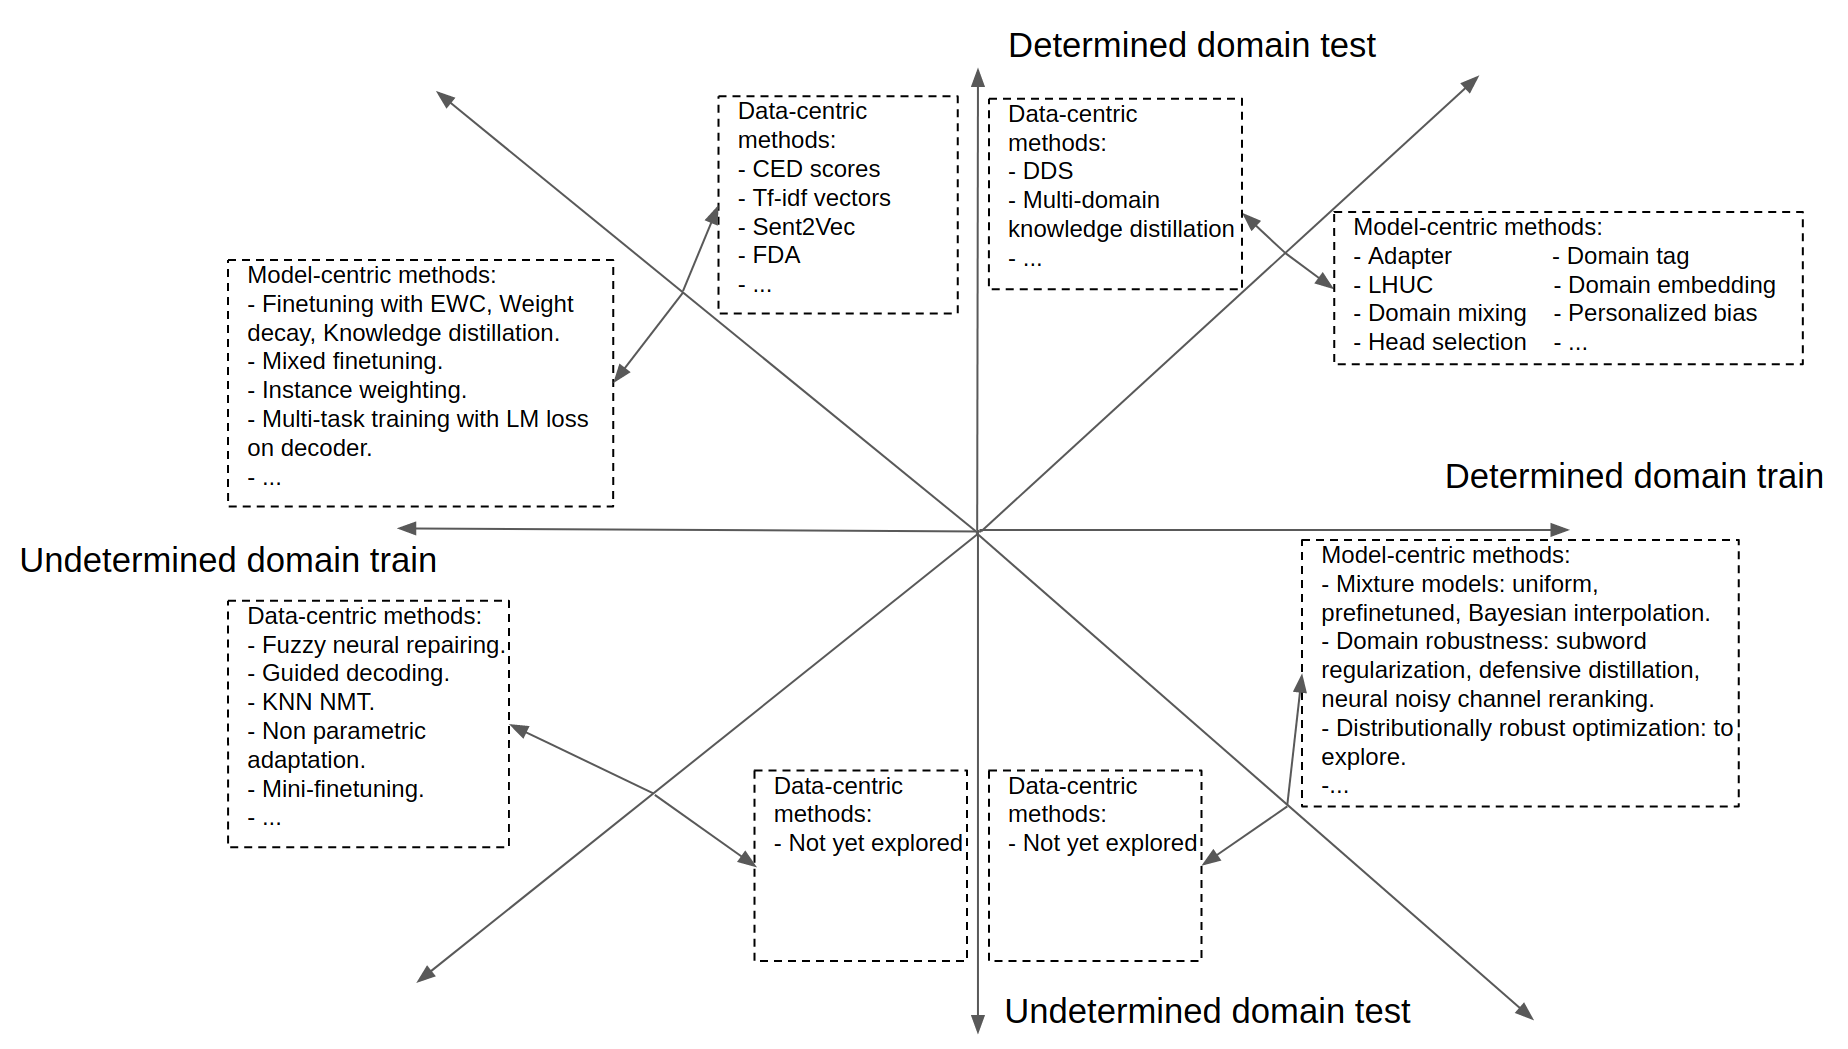
\includegraphics[width=1.2\textwidth]{graphics/review_mdmt}}
  \caption{A complete overview of multi-domain adaptation with the four primary settings and the two groups of approaches.}
\label{fig:review_mdmt}
\end{figure}

This thesis mainly focuses on the first setting in which domain train and domain test are determined. We will present our most important contribution to the study in this setting in the next chapter. This work presents a novel multi-criteria evaluation, which requires five primary properties for a multi-domain system, and reevaluates a wide range of popular model-centric methods with our experimental setting designed to evaluate these five criteria. In Chapter ~\ref{chap:priming}, we study different approaches for the last setting in which domain train and domain test are unspecified.









































































































































































































































































































































































